\documentclass[a4paper]{article}

\usepackage[english]{babel}
\usepackage{amsmath}
\usepackage{amssymb}
\usepackage{dsfont}
\usepackage{tikz}
\usetikzlibrary{arrows,automata}
\title{Calculus and Probability Theory\\ Assignment 7}
\author{Christoph Schmidl\\
s4226887\\
Informatica\\
c.schmidl@student.ru.nl\\
Exercise Teacher: Gergely Alp\'{a}r}

\date{\today}

\begin{document}
\maketitle

\begin{enumerate}

\item (\textbf{20 points}) An experiment consists of drawing 3 cards in succession from a well-shuffled ordinary deck of cards (standard 52-card deck). Let $A_1$ denote the event "Ace on first draw", $A_2$ the event "Ace on second draw" and $A_3$ the event "Ace on third draw". State in words the meaning of each of the following probabilities.








\begin{enumerate}
	\item[(a)] $P(A_1 \cap \neg A_2)$\\
	\textbf{Solution:}\\
	
	
The probability to draw an Ace on the first draw and to draw no Ace on second draw.\\
You can also say: The probability to draw an Ace on the first draw and to draw anything else except an Ace on the second draw.\\		
	
	
	\item[(b)] $P(A_1 \cup A_2)$\\
	\textbf{Solution:}\\

The probability to draw an Ace on the first draw or an Ace on second draw.\\
	
	
	
	\item[(c)] $P(\neg A_1 \cap \neg A_2 \cap \neg A_3)$\\
	\textbf{Solution:}\\
	

The probability to draw no Ace on first draw and no Ace on second draw and no Ace on third draw.\\
You can also say: The probability to draw anything in the first three draws except aces.\\


	
	\item[(d)] $P[(A_1 \cap \neg A_2) \cup (\neg A_2 \cap A_3)]$\\
	\textbf{Solution:}\\
	
The probability to draw an ace on first draw and no Ace on second draw or to draw no ace on second draw and an ace on third draw.\\

	
	
	
	
	\item[(e)] $P(\neg A_1 \cup \neg A_2 | A_1)$\\
	\textbf{Solution:}\\
	
The probability to draw no ace on first draw or no ace on second draw, given that an Ace has already been drawn on first draw.\\	
	
	
	
\end{enumerate}


\item \textbf{(25 points)} Compute the probabilities (a)-(e) in Exercise 1.\\

\begin{align*}
P(A|B) = \frac{P(A \cap B)}{P(B)}\\
P(A|B) \cdot P(B) = P(A \cap B)\\
P(A \cup B) = P(A) + P(B) - P(A \cap B)
\end{align*}


\begin{enumerate}
	\item[(a)] 
	\begin{align*}
P(A_1 \cap \neg A_2) &= P(\neg A_2| A_1) \cdot P(A_1)\\
&= \frac{48}{51} \cdot \frac{4}{52}\\
&= \frac{16}{221}\\
&\approx 0.0724
\end{align*}		
	

	\item[(b)] 
\begin{align*}
P(A_1 \cup A_2) &= P(A_1) + P(A_2) - P(A_1 \cap A_2)\\
&= \frac{4}{52} + \frac{4}{51} - (\frac{4}{52} * \frac{3}{51})\\
&= \frac{100}{664}\\
&\approx 0.1508
\end{align*}	



	
	\item[(c)]
\begin{align*}
P(\neg A_1 \cap \neg A_2 \cap \neg A_3) &= P(\neg A_2 \cap \neg A_3| \neg A_1) \cdot P(\neg A_1)\\
&= (\frac{47}{51} \cdot \frac{46}{50})\cdot \frac{48}{52}\\
&= \frac{1081}{1275} \cdot \frac{48}{52}\\
&= \frac{4324}{5525}\\
&\approx 0.7826
\end{align*}	

\newpage	
	
	
	\item[(d)] 
\begin{align*}
P[(A_1 \cap \neg A_2) \cup (\neg A_2 \cap A_3)] &=\\P(A_1 \cap \neg A_2) + P(\neg A_2 \cap A_3) - P[(A_1 \cap \neg A_2) \cap (\neg A_2 \cap A_3)] &=\\(\frac{4}{52} \cdot \frac{48}{51}) + (\frac{48}{51} \cdot \frac{4}{50}) - (\frac{4}{52} \cdot \frac{48}{51} \cdot \frac{3}{50}) &=\\\frac{792}{5525} &\approx\\0.1433
\end{align*}	
	
	
	\item[(e)]
\begin{align*}
P(\neg A_1 \cup \neg A_2 | A_1) &= \frac{(\neg A_1 \cup \neg A_2) \cap A_1}{P(A_1)}\\
&= \frac{\frac{4}{52} \cdot \frac{48}{51}}{\frac{4}{52}}\\
&= \frac{16}{17}\\
&\approx 0.9411
\end{align*}	 
\end{enumerate}






\item \textbf{(20 points)} Assume that a pair of fair dice are to be tossed, and let the random variable X denote the sum of the points.\\


\begin{enumerate}
	\item[(a)] Make a table of the probability function containing the possible values of X and their probabilities.\\
	\textbf{Solution:}\\
	
Sum of dice:\\

\begin{tabular}{l*{6}{c}r}
                  & 1  & 2 & 3 & 4 & 5 & 6 \\
\hline
                 1 \vline & 2 & 3 & 4 & 5 & 6 & 7  \\
                2 \vline  & 3 & 4 & 5 & 6 & 7 & 8  \\
                3 \vline  & 4 & 5 & 6 & 7 & 8 & 9  \\
                4 \vline  & 5 & 6 & 7 & 8 & 9 & 10  \\
                5 \vline  & 6 & 7 & 8 & 9 & 10 & 11  \\
                6 \vline  & 7 & 8 & 9 & 10 & 11 & 12  \\
\end{tabular}

\vspace{1em}
Probabilities of values:\\

\begin{tabular}{l*{12}{c}r}
                   2 & 3 & 4 & 5 & 6 & 7 & 8 & 9 & 10 & 11 & 12\\
\hline
                  $\frac{1}{36}$ & $\frac{1}{18}$ & $\frac{1}{12}$ & $\frac{1}{9}$ & $\frac{5}{36}$ & $\frac{1}{6}$ & $\frac{5}{36}$ & $\frac{1}{9}$ &  $\frac{1}{12}$ & $\frac{1}{18}$ & $\frac{1}{36}$  \\
\end{tabular}
\vspace{1em}


\newpage
	
	\item[(b)] Draw a histogram of this probability function.\\
	\textbf{Solution:}\\
	
	\begin{figure}[ht]
	\centering
  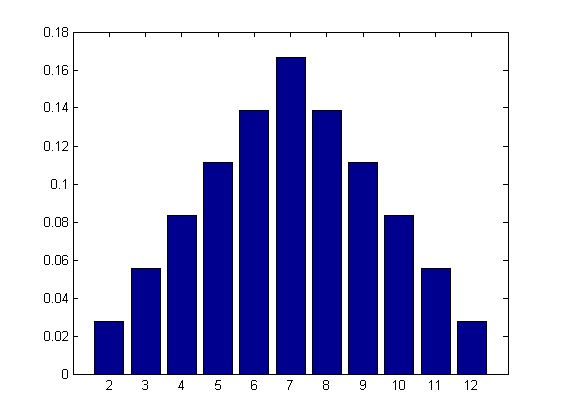
\includegraphics[width=0.8\textwidth]{pdf.png}
\end{figure}	
	
	\item[(c)] What is $P(X\; is\; even)$?\\
	\textbf{Solution:}
	
\begin{align*}
P(X\; is\; even) &= P(X = 2)+P(X = 4)+P(X = 6)\\& +P(X = 8)+P(X = 10)+P(X = 12)\\
&= 	\frac{1}{36} + \frac{1}{12} + \frac{5}{36} + \frac{5}{36} + \frac{1}{12} + \frac{1}{36}\\
&= \frac{1}{2}\\
&= 0.5
\end{align*}	
	
	\item[(d)] What is $P(X \; is \; even|X = 2)$?\\
	\textbf{Solution:}\\

\begin{align*}
P(X \; is \; even|X = 2) &= \frac{P(X \; is \; even \cap X = 2)}{P(X = 2)}\\	
&= \frac{\frac{1}{36}}{\frac{1}{36}}\\
&= 1
\end{align*}	

\newpage	
	\item[(d)] What is $P(X = 2| X \; is \; even)$?\\
	\textbf{Solution:}\\
	
\begin{align*}
P(X = 2 | X \; is \; even) &= \frac{P(  X = 2 \cap X \; is \; even)}{P(X \; is \; even)}\\
&= \frac{\frac{1}{36}}{\frac{1}{2}}\\
&= \frac{1}{18}\\
&\approx 0.055
\end{align*}	
	
	
	
\end{enumerate}



\item \textbf{(20 points)} If $10\%$ of the bolts produced by a machine are defective, determine the following probabilities.

\begin{enumerate}
	\item[(a)] Out of four bolts chosen at random 1 bolt will be defective.\\
	\textbf{Solution:}\\
	
We have $n = 4$, defective probability $p = \frac{1}{10}$ and one bolt defective.	
	
\begin{align*}
	b(1) &= {4 \choose 1}(\frac{1}{10})^1(\frac{9}{10})^3\\
	&= \frac{4}{10} \cdot \frac{729}{1000}\\
	&= \frac{729}{2500}\\
	&\approx 0.2916
\end{align*}

The probability that out of four bolts chosen at random, 1 bolt will be defective, is $29.16\%$.\\
	
	
	\item[(b)] Out of four bolts chosen at random 0 bolt will be defective.\\
	\textbf{Solution:}\\
	
We have $n = 4$, defective probability $p = \frac{1}{10}$ and 0 bolt defective.	
	
\begin{align*}
	b(0) &= {4 \choose 0}(\frac{1}{10})^0(\frac{9}{10})^4\\
	&= 1 \cdot \frac{6561}{10000}\\
	&\approx 0.6561
\end{align*}

The probability that out of four bolts chosen at random, 0 bolts will be defective, is $65.61\%$.\\



	
	
	
	\item[(c)] Out of four bolts chosen at random less than 2 bolts will be defective.\\
	\textbf{Solution:}\\

We can just add the probabilities from (a) and (b)here:\\

\begin{align*}
P = \frac{6561}{10000} + \frac{729}{2500} \approx 0.9477
\end{align*}
	
	
	\item[(d)] Out of four bolts chosen at random 2,3 or 4 bolts are defective.\\
	\textbf{Solution:}\\
	
\begin{align*}
b(2) + b(3) + b(4) &= {4 \choose 2}(\frac{1}{10})^2(\frac{9}{10})^2 + {4 \choose 3}(\frac{1}{10})^3(\frac{9}{10})^1 + {4 \choose 4}(\frac{1}{10})^4(\frac{9}{10})^0\\
&= \frac{243}{5000} + \frac{9}{2500} + \frac{1}{10000}\\
&= \frac{523}{10000}\\
&= 0.0523
\end{align*}	
	
	
	
\end{enumerate}



\item \textbf{(15 points)} Urn A has 2 white and 3 red balls. Urn B has 4 white and 1 red ball. And Urn C has 3 white and 4 red balls. An urn is selected at random and a ball drawn at random is found to be white. Find the probability that Urn A was selected.\\
\textbf{Solution:}\\

There are 17 balls in total. 9 white balls and 8 red balls.


Urn A: 

\begin{itemize}
	\item 5 balls in total $\rightarrow \frac{5}{17}$ of all balls
	\item 2 white balls $\rightarrow \frac{2}{9}$ of all white balls $\rightarrow \frac{2}{5}$ of all balls in Urn A are white
	\item 3 red balls $\rightarrow \frac{3}{8}$ of all red balls $\rightarrow \frac{3}{5}$ of all balls in Urn A are red
\end{itemize}


Urn B: 

\begin{itemize}
	\item 5 balls in total $\rightarrow \frac{5}{17}$ of all balls
	\item 4 white balls $\rightarrow \frac{4}{9}$ of all white balls $\rightarrow \frac{4}{5}$ of all balls in Urn B are white
	\item 1 red balls $\rightarrow \frac{1}{8}$ of all red balls $\rightarrow \frac{1}{5}$ of all balls in Urn B are red
\end{itemize}

Urn C: 

\begin{itemize}
	\item 7 balls in total $\rightarrow \frac{7}{17}$ of all balls
	\item 3 white balls $\rightarrow \frac{3}{9}$ of all white balls $\rightarrow \frac{3}{7}$ of all balls in Urn C are white
	\item 4 red balls $\rightarrow \frac{4}{8}$ of all red balls $\rightarrow \frac{4}{7}$ of all balls in Urn C are red
\end{itemize}

If you draw a ball at random then the chance that it came from Urn A is $\frac{5}{17}$\\

Question reformulated: 

\begin{align*}
P(Urn \; A \; selected | Ball = white) &= \frac{P(Ball = white | Urn \; A \; selected)\cdot P(Urn \; A \; selected)}{P(Ball = white)}\\
&= \frac{\frac{2}{5} \cdot \frac{1}{3}}{\frac{9}{17}}\\
&= \frac{\frac{2}{15}}{\frac{9}{17}}\\
&= \frac{34}{135}\\
&\approx 0.2519
\end{align*}






	
\end{enumerate}

\end{document}
